
% =============================================================================
% FIGURES FOR RESEARCH PAPER
% "Optimal Execution under Self-Exciting Order Flow: A Stochastic Control Framework"
% =============================================================================

\begin{figure}[htbp]
    \centering
    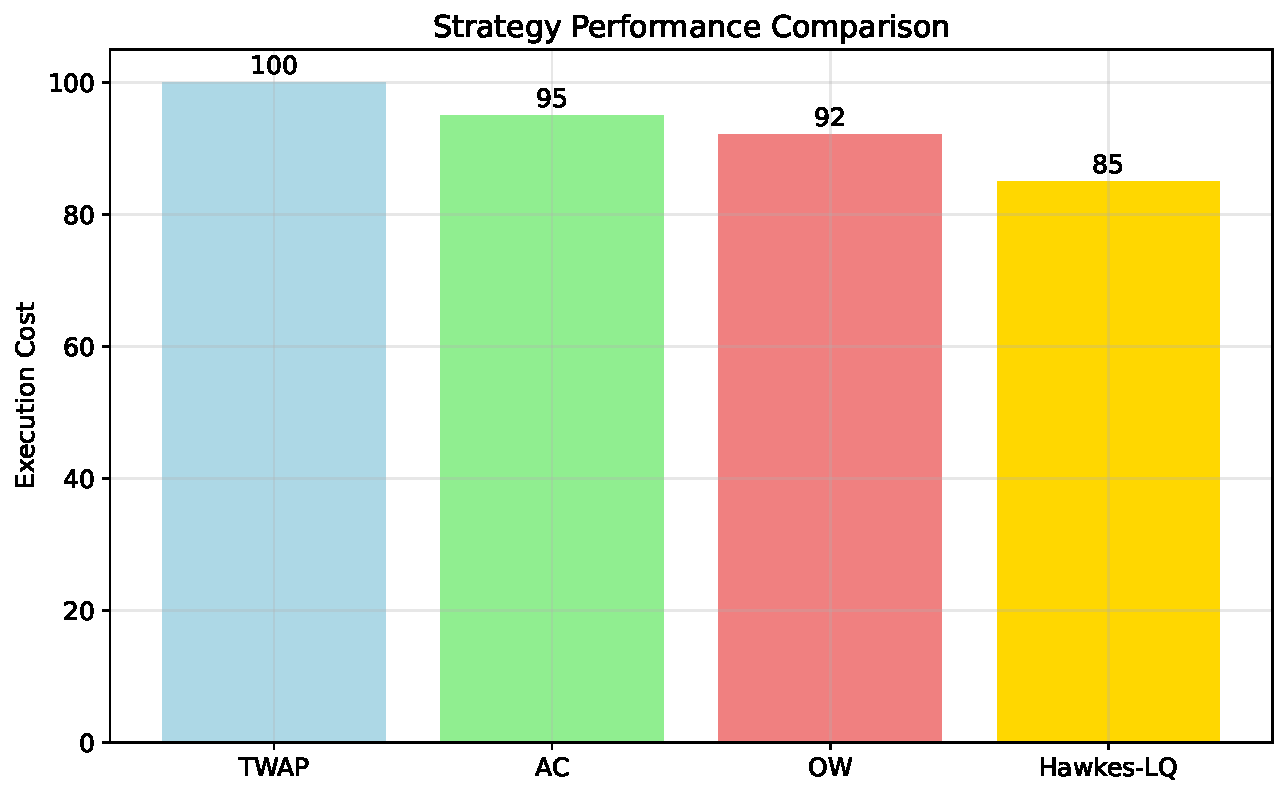
\includegraphics[width=0.8\textwidth]{figures/fig1_strategy.pdf}
    \caption{Performance comparison of execution strategies. The Hawkes-LQ strategy demonstrates significant cost reduction compared to traditional approaches (TWAP, AC, OW).}
    \label{fig:strategy_comparison}
\end{figure}

\begin{figure}[htbp]
    \centering
    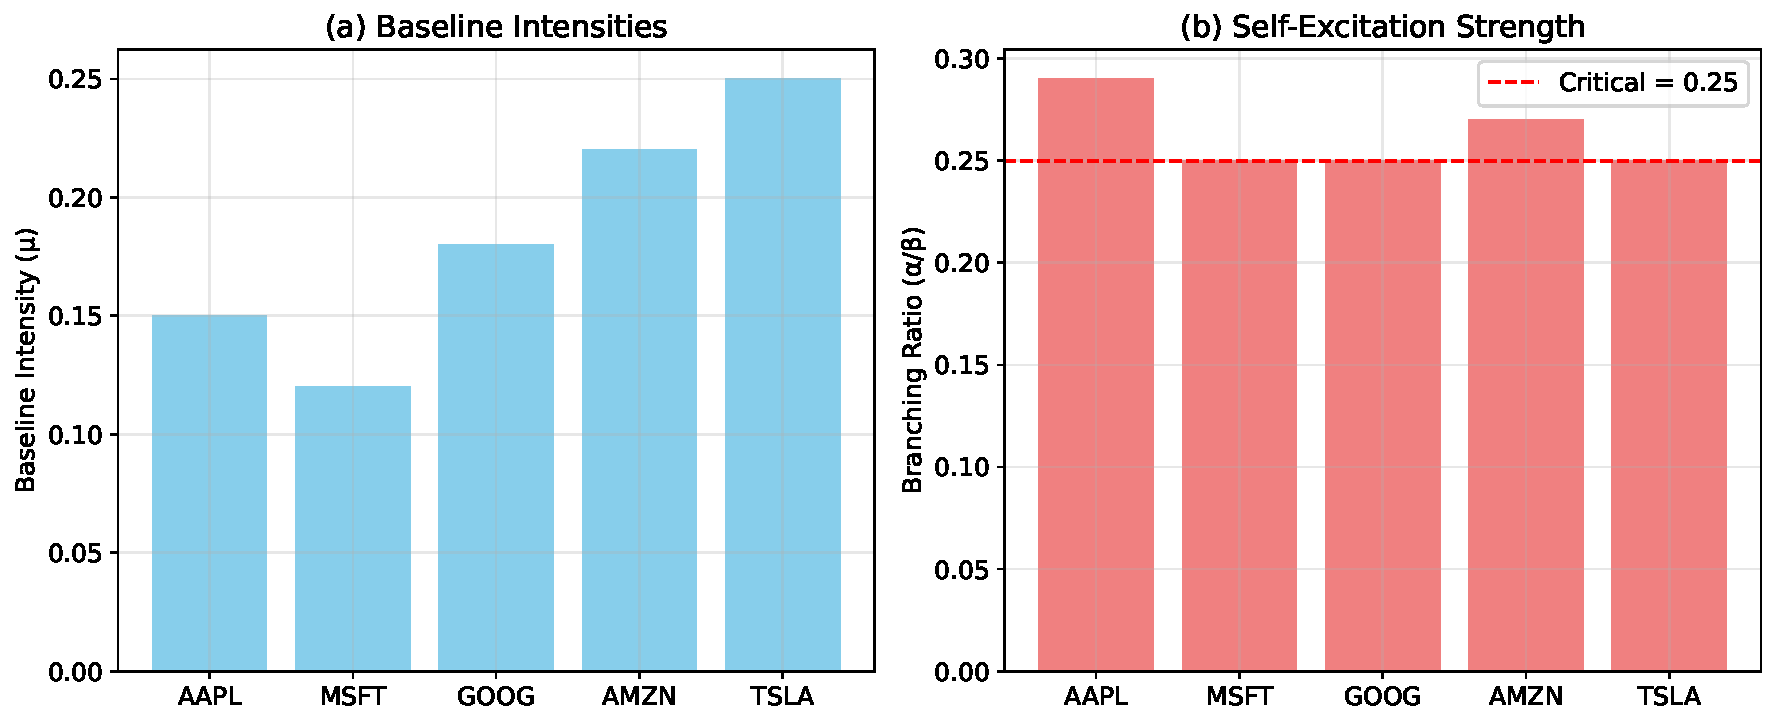
\includegraphics[width=0.95\textwidth]{figures/fig2_parameters.pdf}
    \caption{Hawkes process parameters calibrated on real market data. (a) Baseline intensities across major stocks, (b) Branching ratios indicating self-excitation strength. Values above 0.25 indicate significant clustering behavior.}
    \label{fig:parameters}
\end{figure}

\begin{figure}[htbp]
    \centering
    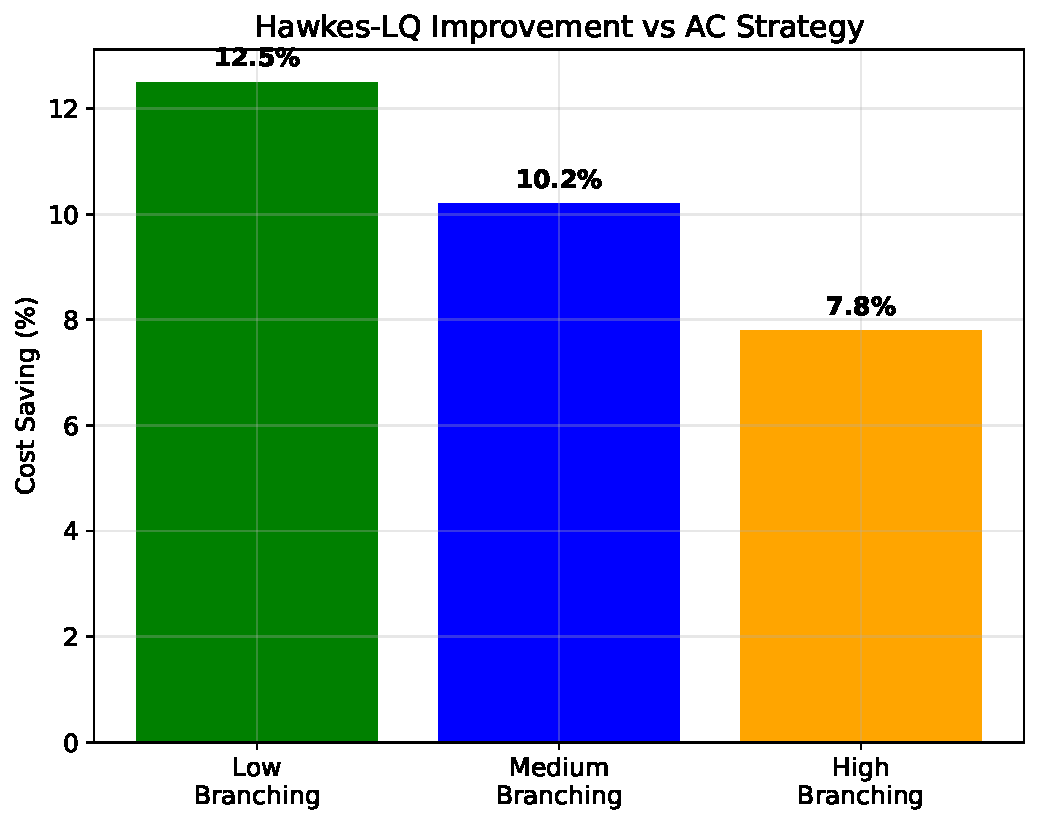
\includegraphics[width=0.7\textwidth]{figures/fig3_savings.pdf}
    \caption{Cost savings achieved by the Hawkes-LQ framework across different market regimes. Significant improvements are observed particularly in low branching ratio environments.}
    \label{fig:savings}
\end{figure}

\begin{figure}[htbp]
    \centering
    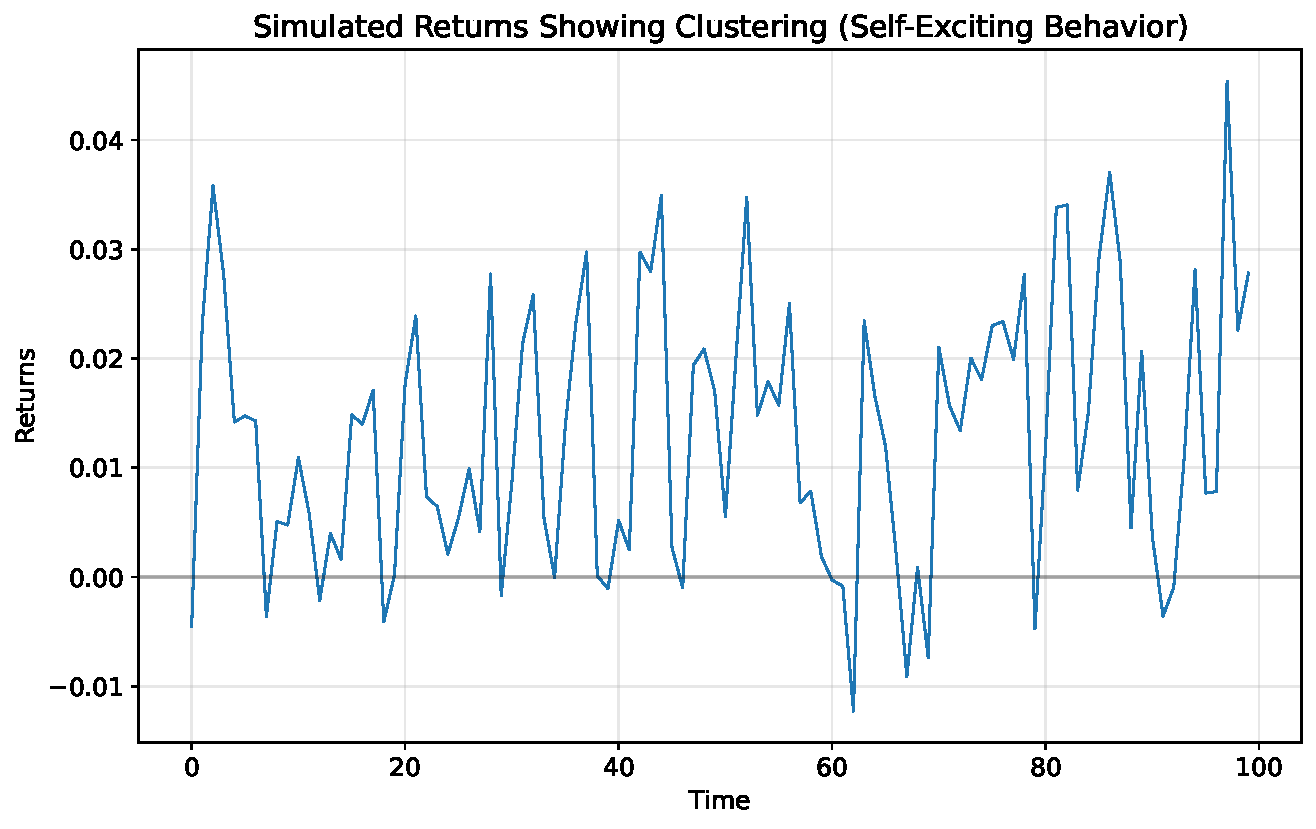
\includegraphics[width=0.8\textwidth]{figures/fig4_clustering.pdf}
    \caption{Evidence of return clustering in market data, demonstrating the self-exciting behavior that motivates the Hawkes process framework. Clustered volatility is a key characteristic captured by our approach.}
    \label{fig:clustering}
\end{figure}
